\documentclass[dvipsnames,tikz,border=0.14mm]{standalone}
\usepackage{tikz}

\newcommand*{\peperoni}[3]{
  \pgfmathsetmacro{\x}{#1}
  \pgfmathsetmacro{\y}{#2}
  \pgfmathsetmacro{\deg}{#3}
  \fill[BrickRed] (\x,\y) circle (0.07);
  \fill[Salmon,rotate around={\deg+45:(\x,\y)}] (\x+0.03,\y-0.02) ellipse (0.008 and 0.006);
  \fill[Salmon,rotate around={\deg+95:(\x,\y)}] (\x+0.04,\y-0.01) ellipse (0.012 and 0.009);
  \fill[Salmon,rotate around={\deg+200:(\x,\y)}] (\x+0.02,\y+0.02) ellipse (0.008 and 0.005);
  \fill[Salmon,rotate around={\deg+300:(\x,\y)}] (\x-0.03,\y-0.02) ellipse (0.005 and 0.007);
  \fill[Salmon,rotate around={\deg+320:(\x,\y)}] (\x+0.04,\y-0.02) ellipse (0.010 and 0.008);
}

\newcommand*{\olive}[2]{
  \draw[Black] (#1,#2) circle (0.022);
}

\newcommand*{\greenpepper}[3]{
  \pgfmathsetmacro{\x}{#1}
  \pgfmathsetmacro{\y}{#2}
  \pgfmathsetmacro{\deg}{#3}
  \begin{scope}[rotate around={\deg:(\x,\y)}]
    \draw[ForestGreen!50!Black,xshift=0.2,yshift=-0.1] plot [smooth,tension=1.2] coordinates {
      (\x,\y-0.005) (\x+0.01,\y+0.01) (\x+0.02,\y) (\x+0.04,\y+0.03) (\x+0.06,\y) (\x+0.07,\y+0.01) (\x+0.08,\y-0.005)
    };
    \draw[Green] plot [smooth,tension=1.2] coordinates {
      (\x,\y-0.005) (\x+0.01,\y+0.01) (\x+0.02,\y) (\x+0.04,\y+0.03) (\x+0.06,\y) (\x+0.07,\y+0.01) (\x+0.08,\y-0.005)
    };
  \end{scope}
}

\newcommand*{\mushroom}[3]{
  \pgfmathsetmacro{\x}{#1}
  \pgfmathsetmacro{\y}{#2}
  \pgfmathsetmacro{\deg}{#3}
  \begin{scope}[rotate around={\deg:(\x,\y)}]
    \fill[Tan] plot [smooth,tension=1.1] coordinates {
      (\x+0.03,\y-0.04) (\x+0.02,\y) (\x+0.05,\y) (\x+0.03,\y+0.04)
      (\x-0.03,\y+0.04) (\x-0.05,\y) (\x-0.02,\y) (\x-0.03,\y-0.04)
    };
  \end{scope}
}

\begin{document}
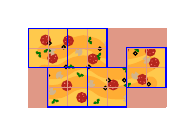
\begin{tikzpicture}
  % Background
  \fill[Yellow!70!Red!70!White] (0,0) rectangle (1.75,1);

  % Sauce
  \draw[Yellow!60!Red!80!White,line width=5,line cap=round] plot [smooth,tension=0.8] coordinates {
    (0.2,0.2) (0.4,0.2) (0.6,0.3) (0.8,0.3) (1,0.2) (1.3,0.2) (1.55,0.3)
  };
  \draw[Yellow!60!Red!80!White,line width=5,line cap=round] plot [smooth,tension=0.8] coordinates {
    (0.2,0.45) (0.4,0.45) (0.6,0.55) (0.8,0.55) (1,0.45) (1.3,0.45) (1.55,0.55)
  };
  \draw[Yellow!60!Red!80!White,line width=5,line cap=round] plot [smooth,tension=1.1] coordinates {
    (0.2,0.7) (0.4,0.7) (0.6,0.8) (0.8,0.8) (1,0.7) (1.3,0.7) (1.55,0.8)
  };

  % Toppings
  \peperoni{0.12}{0.37}{229}
  \peperoni{0.15}{0.13}{30}
  \peperoni{0.22}{0.85}{499}
  \peperoni{0.31}{0.62}{100}
  \peperoni{0.49}{0.27}{771}
  \peperoni{0.51}{0.84}{183}
  \peperoni{0.68}{0.12}{500}
  \peperoni{0.82}{0.61}{401}
  \peperoni{1.08}{0.28}{182}
  \peperoni{1.21}{0.73}{68}
  \peperoni{1.44}{0.11}{99}
  \peperoni{1.45}{0.35}{221}
  \peperoni{1.55}{0.71}{255}
  \peperoni{1.60}{0.56}{129}

  \olive{0.13}{0.31}
  \olive{0.25}{0.4}
  \olive{0.27}{0.81}
  \olive{0.45}{0.76}
  \olive{0.48}{0.51}
  \olive{0.77}{0.51}
  \olive{0.91}{0.74}
  \olive{0.98}{0.24}
  \olive{1.02}{0.34}
  \olive{1.11}{0.83}
  \olive{1.22}{0.34}
  \olive{1.36}{0.68}
  \olive{1.53}{0.29}

  \mushroom{0.3}{0.2}{200};
  \mushroom{0.3}{0.7}{20};
  \mushroom{0.4}{0.4}{60};
  \mushroom{0.64}{0.7}{260};
  \mushroom{0.8}{0.3}{170};
  \mushroom{1.01}{0.8}{270};
  \mushroom{1.25}{0.1}{330};
  \mushroom{1.36}{0.4}{140};
  \mushroom{1.50}{0.6}{221};
  \mushroom{1.62}{0.15}{290};

  \greenpepper{0.1}{0.7}{310}
  \greenpepper{0.2}{0.7}{10}
  \greenpepper{0.3}{0.05}{20}
  \greenpepper{0.5}{0.5}{0}
  \greenpepper{0.7}{0.4}{160}
  \greenpepper{0.8}{0.8}{100}
  \greenpepper{0.9}{0.1}{220}
  \greenpepper{0.9}{0.6}{80}
  \greenpepper{1.0}{0.5}{30}
  \greenpepper{1.1}{0.8}{100}
  \greenpepper{1.2}{0.5}{310}
  \greenpepper{1.3}{0.3}{200}
  \greenpepper{1.4}{0.7}{110}
  \greenpepper{1.5}{0.8}{190}
  \greenpepper{1.6}{0.2}{260}

  % Grid lines
  \draw[Brown!50!Apricot!70!White,ultra thin] (0,0) grid[step=0.25] (1.75,1);

  % Cover some pieces as in sample 1
  \fill[Brown!50!Apricot!70!White] (0,0) rectangle (0.25,0.5);
  \fill[Brown!50!Apricot!70!White] (1,0.5) rectangle (1.25,1);
  \fill[Brown!50!Apricot!70!White] (1,0.75) rectangle (1.75,1);
  \fill[Brown!50!Apricot!70!White] (1.25,0) rectangle (1.75,0.25);

  % Draw the 2x2 squares
  \draw[Blue] (0,0.5) rectangle (0.5,1.0);
  \draw[Blue] (0.25,0) rectangle (0.75,0.5);
  \draw[Blue] (0.5,0.5) rectangle (1.0,1.0);
  \draw[Blue] (0.75,0) rectangle (1.25,0.5);
  \draw[Blue] (1.25,0.25) rectangle (1.75,0.75);
\end{tikzpicture}
\end{document}

